\documentclass[12pt]{article}
\usepackage[czech]{babel}
\usepackage[utf8]{inputenc}
\usepackage[IL2]{fontenc}
\usepackage{wrapfig}
\usepackage{graphicx}
\usepackage{cprotect}
\usepackage{amsmath}


\begin{document}
%\setlength{\parindent}{0pt}
\begin{titlepage}

\includegraphics[scale=0.2, trim=5cm 0 0 30cm]{logo.jpg}
\begin{center}
\vspace{5cm}
{\Huge
\textbf{KIV/MKZ}\\
\vspace{1cm}
}
{\Large
\textbf{To Do List}
}
\end{center}
\vspace{\fill}

\begin{minipage}[t]{5cm}
\flushleft
Martin Hamet\\
\end{minipage}
\hfill
\begin{minipage}[t]{7cm}
\flushright
\today
\end{minipage}
\end{titlepage}

\tableofcontents
\newpage
\section{Zadání}
\label{zadani}
Vytvořte aplikaci pro mobilní zařízení na platformě Android. Aplikace bude typu "To Do List". Měla by poskytovat možnost zadání, úpravy, řazení a dokončení úlohy.

\section{Analýza problému a návrh řešení}
Úkolem je vytvořit praktickou aplikaci, která přehledně zobrazuje úlohy zadané uživatelem. Důraz by měl být kladen na jednoduchost aplikace v takovém smyslu, aby uživatel nebyl nucen ke zbytečným rutinním úkonům, jako je tomu zvykem u aplikací podobného typu. Pokud je činnost s aplikací otravná nebo zdlouhavá uživatel ztrácí zájem o její používání.

\subsection{Úlohy}
Konkrétní úlohou je myšlena jakákoliv aktivita (odeslání emailu, seznam nákupu, schůzka, ...), proto nemá smysl zabývat se výběrem typu jednotlivých úloh. Každá úloha by měla obsahovat časový údaj o jejím datu vypršení. 

Seznam úloh bude řazen podle jejich data. Úlohy, které slouží jako poznámka nepotřebují datum prodlení, nicméně přiřazením aktuálního data můžeme zajistit jejich pozici na začátku seznamu s informací o jejich času vytvoření. Předpokládáme že poznámky nemají dlouhodobý význam a budou dříve odstraňovány.

Především kvůli poznámkám je třeba udržovat informaci s nepovinným obsáhlejším popisem daného úkolu. Podrobné informace s možnostmi změn data a času by měli být v samostatném okně kvůli minimalizaci prvků na obrazovce. 

Editační okno by mělo být přehledné a zajistit výběr data a času pomocí dostupných podpůrných prvků (kalendář, hodiny). Z vlastní zkušenosti s podobnými aplikacemi, aby nedocházelo k ukončování jednotlivých úloh omylem, v hlavním okně, tlačítko pro ukončení by mělo být součástí okna pro editaci. 

Z hlediska neobtěžování uživatele ovládáním, potvrzovacími dialogy, nastavováním jednotlivých úkolů, atp. omezíme nastavení pouze na tyto jednoduché atributy, které se budou bez vyplnění inicializovat na validní hodnoty (aktuální datum a čas). Samotné potvrzení ukončení úlohy lze také zjednodušit na potvrzení dvojklikem bez dialogu. Podobně není nutné vyžadovat potvrzování editace úlohy.

\subsection{Data}
Uložení seznamu úloh musí být perzistentní nezávisle na běhu aplikace. Nabízí se ukládání do souboru a databáze. Předpokládáme práci s poměrně malým počtem dat nicméně časté čtení a upravování souboru považuji za zbytečně náročné a použití tlačítka pro uložení je proti našemu hlavnímu cíli jednoduchosti ovládání a použijeme tedy perzistentní databázi. Bude potřeba automaticky propagovat změny dat z vnitřních datových struktur do databáze, aby nedošlo ke ztrátě. Pro založení databáze bude vhodné využít \texttt{SQLite} podporovaný platformou. 

Jako vnitřní datovou strukturu bude vhodné použít mapu vzhledem k snadnému přístupu k jednotlivým úlohám podle jejich \texttt{ID}. Protože aplikace využívá více oken bude výhodné navrhnout datovou strukturu s využitím návrhového vzoru \texttt{Design Pattern Singleton}, která bude zajišťovat jednotný přístup k datům a může se starat o vlastní propagaci do databáze.

\subsection{Notifikace}
Upozornění by měla být volitelná služba, která zobrazí upozornění o nesplněných úlohách pro daný den. Protože aplikace není myšlena jako plánovač akcí a měla by sloužit jako nenásilné upozornění na čekající úlohy. Notifikace bude tedy probíhat pouze jednou denně, kdy poskytne zběžný přehled o čekajících úlohách. Z logiky upozorňování služba tvořící notifikace by měla být spouštěna i když aplikace běží pouze na pozadí. Což půjde zařídit nastavením plánovače úloh.

\pagebreak
\section{Implementace (popis řešení)}
V této sekci budou popsány hlavní moduly programu a jejich vzájemná funkce.

\subsection{\texttt{MainActivity}}
Zajišťuje funkčnost hlavního okna aplikace. Jedná se tedy o seřazený seznam jednotlivých úloh s tlačítkem pro zapnutí (vypnutí) notifikací a přidání nové úlohy.

\paragraph{\texttt{onCreate()}}
Naplní list úlohami a nastaví \texttt{Listener} na jeho prvky pro umožnění editace prvku spuštěním aktivity \texttt{TaskAktivity} v módu editace (attribut \texttt{editing = true}).

\paragraph{\texttt{btAdd\_onClick()}}
Umožní přidání nové úlohy spuštěním \texttt{TaskAktivity} s attributem \texttt{editing = false}.

\paragraph{\texttt{scheduleNotifications()}}
Registruje opakované volání služby pro tvoření notifikací \texttt{NotificationService} pomocí \texttt{AlarmManager}. Vypnutí notifikací zajišťuje \texttt{cancelNotification()}.

\subsection{\texttt{TaskAktivity}}
Třída zajišťující funkčnost okna pro editaci nebo přidání úlohy.

\paragraph{\texttt{onCreate()}}
Naplní prvky okna příslušnými hodnotami (hodnoty vybrané úlohy pro editaci, základní hodnoty jinak).

\paragraph{\texttt{addTask()}}
Z hodnot z jednotlivých elementů okna vytvoří novou instanci úlohy, kterou předá do datové struktury.

\subsection{\texttt{TaskList}}
Představuje vnitřní datovou strukturu, poskytuje přístup k datům a stará se o propagaci změn do databáze.

\paragraph{\texttt{getInstance()}}
Vrátí jedinou instanci třídy a při prvním volání provede naplnění datových struktur z databáze.

\paragraph{\texttt{put()}, \texttt{remove()}}
Přidání a odebrání úlohy.

\paragraph{\texttt{update()}}
Zajistí propagaci změn dané úlohy do databáze.

\paragraph{getSortedList()}
Získá seřazený list všech úloh.

\subsection{\texttt{Task}}
Obalová třída reprezentující jednu úlohu s jejími atributy.

\subsection{\texttt{DBHelper}}
Poskytuje rozhraní pro snadný přístup k databázi je využívána pouze z vnitřní datové struktury (\texttt{TaskList}).

\subsection{\texttt{NotificationService}}
Služba zajišťující vytvoření notifikace.

\subsection{\texttt{NotificationServiceReceiver}}
Zajišťuje volání služby \texttt{NotificationService} na podnět plánovače úloh (\texttt{AlarmManager)}.


\pagebreak
\section{Uživatelská příručka}
Pro spuštění programu je třeba minimální platforma Android verze \texttt{JellyBean}. 

\subsection{Hlavní okno}
\begin{wrapfigure}[8]{r}{5cm}
\centering
\vspace{-1.5cm}
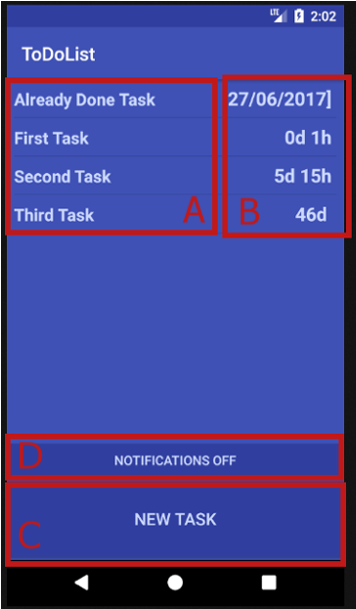
\includegraphics[height=6cm]{MainWindow.png}
\caption{Hlavní okno.}
\label{MainWindow}
\end{wrapfigure}


Hlavní okno obsahuje seznam seřazených úkolů podle data. Editaci jednotlivých úloh lze vyvolat kliknutím na požadovaný prvek. Nový úkol přidáme pomocí tlačítka \texttt{NEW TASK}.

\begin{itemize}
\renewcommand\labelitemi{--}
\setlength\itemsep{1px}
\item{\texttt{A}} Seznam jednotlivých úloh.
\item{\texttt{B}} Zbývající čas do vypršení úlohy.
\item{\texttt{C}} Tlačítko pro přidání nové úlohy.
\item{\texttt{D}} Vypnutí/zapnutí notifikací.
\end{itemize}

\subsection{Okno editace/přidání úlohy}
\begin{wrapfigure}[11]{r}{5cm}
\centering
\vspace{-0.5cm}
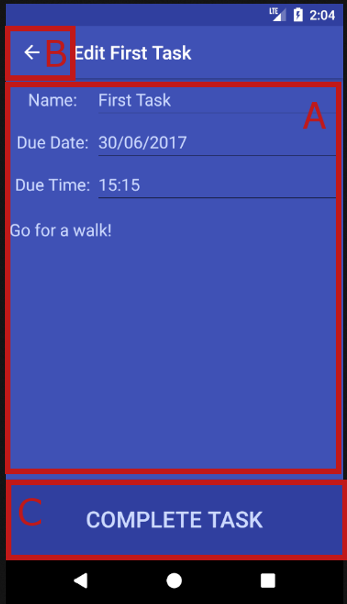
\includegraphics[height=6cm]{EditWindow.png}
\caption{Okno editace.}
\label{EditWindow}
\end{wrapfigure}

Okno editace obsahuje detailní informace zvoleného nebo nového prvku. V případě editace prvku \textbf{dvojklikem} na tlačítko \texttt{COMPLETE TASK} úlohu ukončíme. Kliknutím na datum/čas vyvoláme komponentu pro výběr data/času.

\begin{itemize}
\renewcommand\labelitemi{--}
\setlength\itemsep{1px}
\item{\texttt{A}} Informace o zvolené/nové úloze.
\item{\texttt{B}} Tlačítko pro návrat na hlavní obrazovku.
\item{\texttt{C}} Ukončení úlohy/přidání nové úlohy.
\end{itemize}

\section{Testování}
Testování proběhlo ve vývojovém prostředí \texttt{Android Studio} na virtuálních strojích \texttt{Nexus 5 API 25} a \texttt{Nexus 5X API 25}. Dále na vlastním zařízení \texttt{Xperia L CZ105} s verzí \texttt{Android 4.2.2 JellyBean}. 

Při testování bylo odhaleno několik nedostatků týkajících se zobrazení, které byli odstraněny a funkční chyby tlačítka pro zapnutí notifikací.

\section{Závěr}
Program bylo překvapivě náročné zprovoznit přesto že programově náročný není. Většina problémů při vývoji vznikla v souvislosti s komplexností vývojového prostředí a následně jeho konfigurace. Ohledně problému při kódování jde pouze o jiný pohled na běh aplikace co se týče života aktivity a služeb.

Samotná aplikace vyhovuje požadavku na jednoduchost ovládání a je mnohem pohodlnější než předchozí alternativa, kterou jsem používal, kde se často stávalo že se úloha ukončila nechtěným stisknutím tlačítka.
\end{document}